\documentclass[11pt]{article}
% =========================================================================
% SHARED STYLE FILE for 11_Master_Projects reports
% Visual style follows 0_Thesis_Submission/24m0553_AK_Gaurav_Mtech_Report.pdf:
% serif body font, blue hyperlinked TOC/links, ruled section headings,
% IITB-style title page, formal academic report structure.
% =========================================================================

\usepackage[a4paper,margin=1in]{geometry}
\usepackage{xcolor}
\usepackage{graphicx}
\graphicspath{{../images/}}
\usepackage{amsmath,amssymb}
\usepackage{booktabs}
\usepackage{caption}
\usepackage{float}
\usepackage[hidelinks]{hyperref}
\usepackage{titlesec}
\usepackage{enumitem}
\usepackage{setspace}
\usepackage[T1]{fontenc}
\usepackage{lmodern}
\usepackage{microtype}

% Every \includegraphics call is automatically framed with a thin black
% border (matches the printed look of figures/photos/charts in the source
% reports). \oldincludegraphics is kept available for institutional
% logos/seals on title pages, which should remain unframed.
\let\oldincludegraphics\includegraphics
\setlength{\fboxsep}{1pt}
\setlength{\fboxrule}{0.6pt}
\renewcommand{\includegraphics}[2][]{\fbox{\oldincludegraphics[#1]{#2}}}

\definecolor{thesisblue}{RGB}{0,0,205}
\hypersetup{
  colorlinks=true,
  linkcolor=thesisblue,
  urlcolor=thesisblue,
  citecolor=thesisblue,
  filecolor=thesisblue
}

\onehalfspacing
\setlength{\parskip}{6pt}
\setlength{\parindent}{0pt}

\titleformat{\section}
  {\normalfont\Large\bfseries}{\thesection}{1em}{}
\titleformat{\subsection}
  {\normalfont\large\bfseries}{\thesubsection}{1em}{}
\titleformat{\subsubsection}
  {\normalfont\normalsize\bfseries}{\thesubsubsection}{1em}{}

\newcommand{\reportTitlePage}[7]{%
  % #1 = Report title
  % #2 = Course code & name (e.g. "CE 605: Applied Statistics")
  % #3 = Subtitle/topic line (e.g. "Project Report 2: Network Analysis")
  % #4 = Author block (can be multi-line with \\ for group projects)
  % #5 = Supervisor name(s)
  % #6 = Programme line (e.g. "M.Tech in Transportation Systems Engineering")
  % #7 = Month/Year
  \begin{titlepage}
    \centering
    \vspace*{0.5cm}
    {\large\bfseries #2}\par
    \vspace{0.3cm}
    {\Large\bfseries #3}\par
    \vspace{1.2cm}
    {\Huge\bfseries #1}\par
    \vspace{1.5cm}
    \oldincludegraphics[width=3.2cm]{../../assets/iitb_logo.png}\par
    \vspace{1.2cm}
    Submitted by:\par
    \vspace{0.2cm}
    {\bfseries #4}\par
    \vspace{0.8cm}
    Under the Supervision of\par
    \vspace{0.2cm}
    {\bfseries #5}\par
    \vspace{1.2cm}
    #6\par
    Department of Civil Engineering\par
    \textbf{Indian Institute of Technology Bombay}\par
    Mumbai -- 400076, India\par
    \vspace{0.3cm}
    #7\par
  \end{titlepage}
}

\newcommand{\reportAbstract}[1]{%
  \section*{Abstract}
  #1
  \vspace{0.5cm}
}


\title{Land Use Land Cover Change in Singrauli District}
\author{Abhijeet Kumar Gaurav}
\date{}

\begin{document}

\begin{titlepage}
  \centering
  \vspace*{0.5cm}
  {\large\bfseries Exploratory Project}\par
  \vspace{0.3cm}
  {\Large\bfseries B.Tech Civil Engineering}\par
  \vspace{1.2cm}
  {\Huge\bfseries Land Use Land Cover Change in Singrauli District}\par
  \vspace{2cm}
  Submitted by:\par
  \vspace{0.2cm}
  {\bfseries Abhijeet Kumar Gaurav \\ Roll No.\ 20065001}\par
  \vspace{0.8cm}
  Under the Guidance of\par
  \vspace{0.2cm}
  {\bfseries Dr.\ Medha Jha}\par
  \vspace{1.2cm}
  Department of Civil Engineering\par
  \textbf{Indian Institute of Technology (BHU), Varanasi}\par
  Varanasi -- 221005, India\par
  \vspace{0.3cm}
  2022\par
\end{titlepage}

\pagenumbering{roman}

\reportAbstract{
Land Use Land Cover (LULC) classification is a key application of remote sensing for monitoring
the influence of human activity on the physical environment. This study examines LULC change in
the Singrauli coalfield region, spanning parts of Singrauli district (Madhya Pradesh) and
Sonebhadra district (Uttar Pradesh), over a 15-year span (2006--2021), using multi-temporal
Landsat~5 and Landsat~8 imagery. Supervised (maximum-likelihood) classification was performed in
ArcGIS~10.0 over a study area of 11{,}285.56~sq.\ km, delineating six land cover classes: dense
forest, mining areas, settlement/built-up areas, barren land, vegetation and agricultural land,
and water bodies. The analysis shows a pronounced decline in dense forest cover (from 17.94\% in
2006 to 4.53\% in 2021) and in barren land (from 38.71\% to 15.25\%), accompanied by a marked
increase in vegetation and cultivated land (from 23.95\% to 52.62\%) and in built-up area (from
16.33\% to 23.84\%). Mining area also grew substantially in relative terms, reflecting the rapid
expansion of coal mining and associated overburden dumping. Water body extent declined slightly
over the period, attributed to reduced rainfall, siltation from dumpsite runoff, and heavy
extraction for thermal power and mining use. The study concludes that the LULC change observed in
the Singrauli coalfield is primarily driven by the rapid expansion of coal mining and
industrial activity, resulting in significant transformation of the region's fragile ecosystem.

\vspace{0.3cm}
\noindent\textbf{Keywords:} Land Use Land Cover; Remote Sensing; Landsat; Supervised
Classification; ArcGIS; Singrauli Coalfield; Mining-Induced Land Cover Change
}

\newpage
\tableofcontents
\newpage
\pagenumbering{arabic}

\section{Introduction}

Land Use Land Cover (LULC) classification is the process of assigning land cover classes, such
as water, urban areas, woodland, buildings, agriculture, grassland, and highland, to pixels in
satellite imagery, so that the picture can be naturally grouped into meaningful land
cover classes based on the distinctive spectral reflectance of each cover type.

LULC classification of satellite imagery is an important and exclusively studied area within
remote sensing; accurate and appropriate land use/cover detection nonetheless remains a
challenge. LULC classification plays a noteworthy role in the development of regions and
nations: accurate LULC information is vital for urban land planning, agriculture, rural
management, and sustainable development. Land use/land cover is an important indicator of
global environmental change, reflecting the influence of human activity on the physical
environment. Land use/land cover change is a dynamic, widespread, and accelerating process,
mainly driven by natural phenomena and anthropogenic activities, which in turn impact the
natural ecosystem. Remote sensing technology is extensively used to estimate and monitor such
LULC changes, and LULC maps play a significant and prime role in planning, management, and
monitoring programmes at local, regional, and national levels.

\section{About the Landsat Series}

The Landsat series is a joint USGS and NASA-led enterprise for Earth Observation, representing
the world's longest-running system of satellites for moderate-resolution optical remote sensing
of land, coastal areas, and shallow waters. The first Landsat mission was launched in 1972 as
the first Earth Observation satellite with the goal of monitoring the world's land, and was
followed by successive missions; Landsat-6 failed to achieve orbit and communication with it was
never established, but the series otherwise continues to this day, making Landsat the longest
continuous Earth-imaging programme in history.

\begin{itemize}
  \item \textbf{Landsat-1 to 3:} Landsat-1 was launched in 1972 as the first Earth observation
  satellite with the goal of monitoring the world's land, followed by Landsat-2 in 1975 and
  Landsat-3 in 1978.
  \item \textbf{Landsat-4 and 5:} Landsat-4 was launched in 1982 and Landsat-5 in 1984, carrying
  the Multi-Spectral Scanner and Thematic Mapper instruments.
  \item \textbf{Landsat-7:} launched in 1999, carrying the Enhanced Thematic Mapper Plus 8-band
  whiskbroom scanning radiometer instrument.
  \item \textbf{Landsat-8:} launched in 2013, carrying the Operational Land Imager and Thermal
  Infrared Sensor instrument.
\end{itemize}

\subsection*{Data Used}

\textbf{Landsat 8} (for the years 2016 and 2021): Landsat~8 OLI is one of the most widely used
remote sensing datasets for LULC classification, providing 11 spectral bands. In this study,
bands 1 to 7, namely coastal, blue, green, red, near-infrared (NIR), shortwave infrared~I (SWIR1),
and shortwave infrared~II (SWIR2), were selected for analysis, as bands 8 to 11 are less used
in LULC classification.

\textbf{Landsat 5} (for the years 2006 and 2011): Landsat~5 was a low Earth orbit satellite
launched on 1 March 1984 to collect imagery of the Earth's surface. Jointly managed by USGS and
NASA as a continuation of the Landsat Program, Landsat~5 carried the same Thematic Mapper and
Multi-Spectral Scanner instruments as Landsat~4.

\section{Study Area}

The study area falls within the geo-coordinates 24\textdegree00' to 24\textdegree15' N latitude
and 82\textdegree30' to 82\textdegree45' E longitude, lying partly in Singrauli district of
Madhya Pradesh and partly in Sonebhadra district of Uttar Pradesh. The area is well connected by
motorable road with Varanasi (220~km), Mirzapur (215~km), Rewa (206~km), and Sidhi (130~km). The
nearest railway station is Singrauli, on the Chopan--Katni line, which passes parallel to the
northern periphery of the coalfield; Renukoot, 45~km from Singrauli, is also nearby. An area of
11{,}285.56~sq.\ km was selected as the study area for analysis.

\begin{figure}[H]
\centering
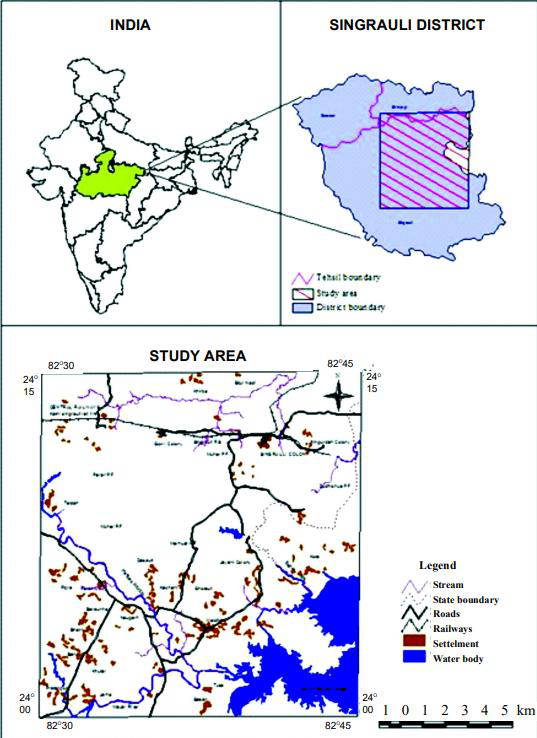
\includegraphics[width=0.88\textwidth]{fig_study_area.png}
\caption{Location map of the study area: India, Singrauli district, and the delineated study
area with settlements, streams, roads, railways, and water bodies.}
\end{figure}

\section{Methodology and Application}

The classification was performed using \textbf{ArcGIS~10.0}, a family of client software,
server software, and online GIS services developed and maintained by Esri; ArcMap within
ArcGIS~10.0 was used to carry out the classification.

Supervised classification is commonly used for LULC analysis, and ArcGIS provides extensive
facilities for standard classification, including tools for classifying numerical fields for
graduated symbology. The Interactive Supervised Classification tool was used to accelerate the
maximum-likelihood classification process, allowing a quick preview of the classification result
without separately running the Maximum Likelihood Classification tool.

\textbf{Steps of supervised classification:}
\begin{center}
\small
Composition of bands $\rightarrow$ creating the shapefile $\rightarrow$ extraction of the
required area $\rightarrow$ creating training samples $\rightarrow$ manually classifying pixels
using various band combinations $\rightarrow$ creating the signature file $\rightarrow$
performing maximum-likelihood classification $\rightarrow$ converting the final raster layer to
a vector polygon $\rightarrow$ calculating the area.
\end{center}

\section{Discussion}

The land use/land cover categories delineated in the study area are dense forest, built-up
areas, mining areas, barren land, water bodies, and vegetation (including agricultural land).

\textbf{Dense forest.} Dense forest area is deciphered from the False Colour Composite (FCC)
satellite image by its dim red tone, coarse-to-medium texture, bordering example, and regular to
sporadic shape. Dense forest area covered 17\% (2021~sq.\ km) of the complete region
(11{,}285~sq.\ km) in 2006, falling to 7\% (803~sq.\ km) in 2011 and 4.53\% in 2021, a decline
of around 1218~sq.\ km between 2006 and 2011 alone. Most coal mining activity takes place in the
dense forest area, since much of the coal resource lies beneath it; the decrease in dense forest
is therefore primarily attributed to the removal of trees as the first step in the expansion of
mining activity, removal of forest for infrastructure supporting heavy industrialisation, and
increasing population.

\textbf{Mining areas.} Mining pits are interpreted on the FCC image by their black tone,
medium-to-smooth texture with a linear to curvilinear pattern, and irregular shape; overburden
dumps and thermal power plants can additionally result in loss of agricultural land. Mining
occupied 66.49~sq.\ km (0.5\%) of the study area in 2006, increasing to 169~sq.\ km (1.54\%) in
2011, an increase of 102.92~sq.\ km, as material removed from mining blocks was dumped along
the periphery of the plains, forming artificial landscapes. Mining areas generally lack all
types of vegetation.

\textbf{Settlement / built-up areas.} Settlement area is situated mostly in the central and
south-western regions of the plain area, and is identified on the FCC image by its cyan to
light-grey tone. Settlement area grew substantially between 2006 and 2011, an increase of
around 1356~sq.\ km, driven by the development of the industrial sector (NCL and NTPC), which
required residential colonies, industrial buildings, schools, and community halls, alongside
rising demand for labour that attracted migrants from other states and drove the expansion of
villages, towns, and cities in this industrial belt.

\textbf{Barren land.} Rocky, barren area is located mostly on the northern side of the study
area, identified on the FCC image by its green-to-brownish tone, coarse texture, and irregular
outline. Barren land area changed only slightly during 2006--2016, but its share fell markedly
to 15.25\% by 2021, owing to the expansion of settlement and cropland areas.

\textbf{Vegetation cover and agricultural land.} Cultivated land in the study area is under
Kharif crops, namely wheat, jowar, masoor, and chana, and is recognised on the FCC image by its red
to light-greenish tone, smooth-to-medium texture, non-contiguous pattern, and regular to
sub-regular outline. Over the study period, as people returned to and expanded agricultural
activity, the vegetation and cultivated land share rose from 23.95\% to 52.62\%.

\textbf{Water bodies.} Water bodies are identified on the FCC image by their light-blue to black
tone, smooth texture, and irregular shape. Water body area fell from 281.12~sq.\ km (2.4\%) in
2006 to 263.05~sq.\ km (2.33\%) in 2010/2011, a decrease of about 18.07~sq.\ km, attributed
to a decline in rainfall of roughly 313~mm between 1978 and 2011, siltation from dumpsite
material runoff, and atmospheric dust pollution. The utilisation of water for thermal power
plants and mining activity is also an important cause of water body depletion, since usage
exceeds the storage capacity of the reservoirs, and washed-out material runoff from dumpsites
further blocks natural drainage.

\begin{figure}[H]
\centering
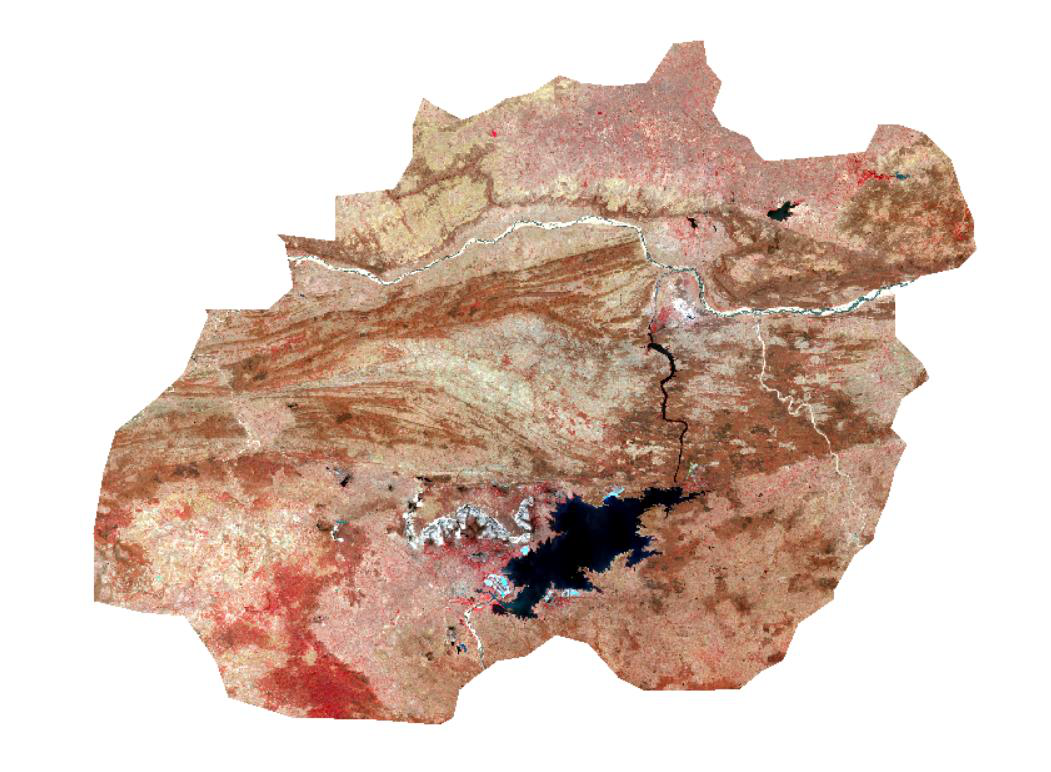
\includegraphics[width=0.92\textwidth]{fig_fcc_composite.png}
\caption{False Colour Composite (FCC) band image of the Singrauli study area.}
\end{figure}

\section{Results}

Figures~2--5 present the classified LULC maps of the Singrauli study area for 2006, 2011, 2016,
and 2021, and Table~\ref{tab:lulc} summarises the corresponding percentage share of each land
cover class over time.

\begin{figure}[H]
\centering
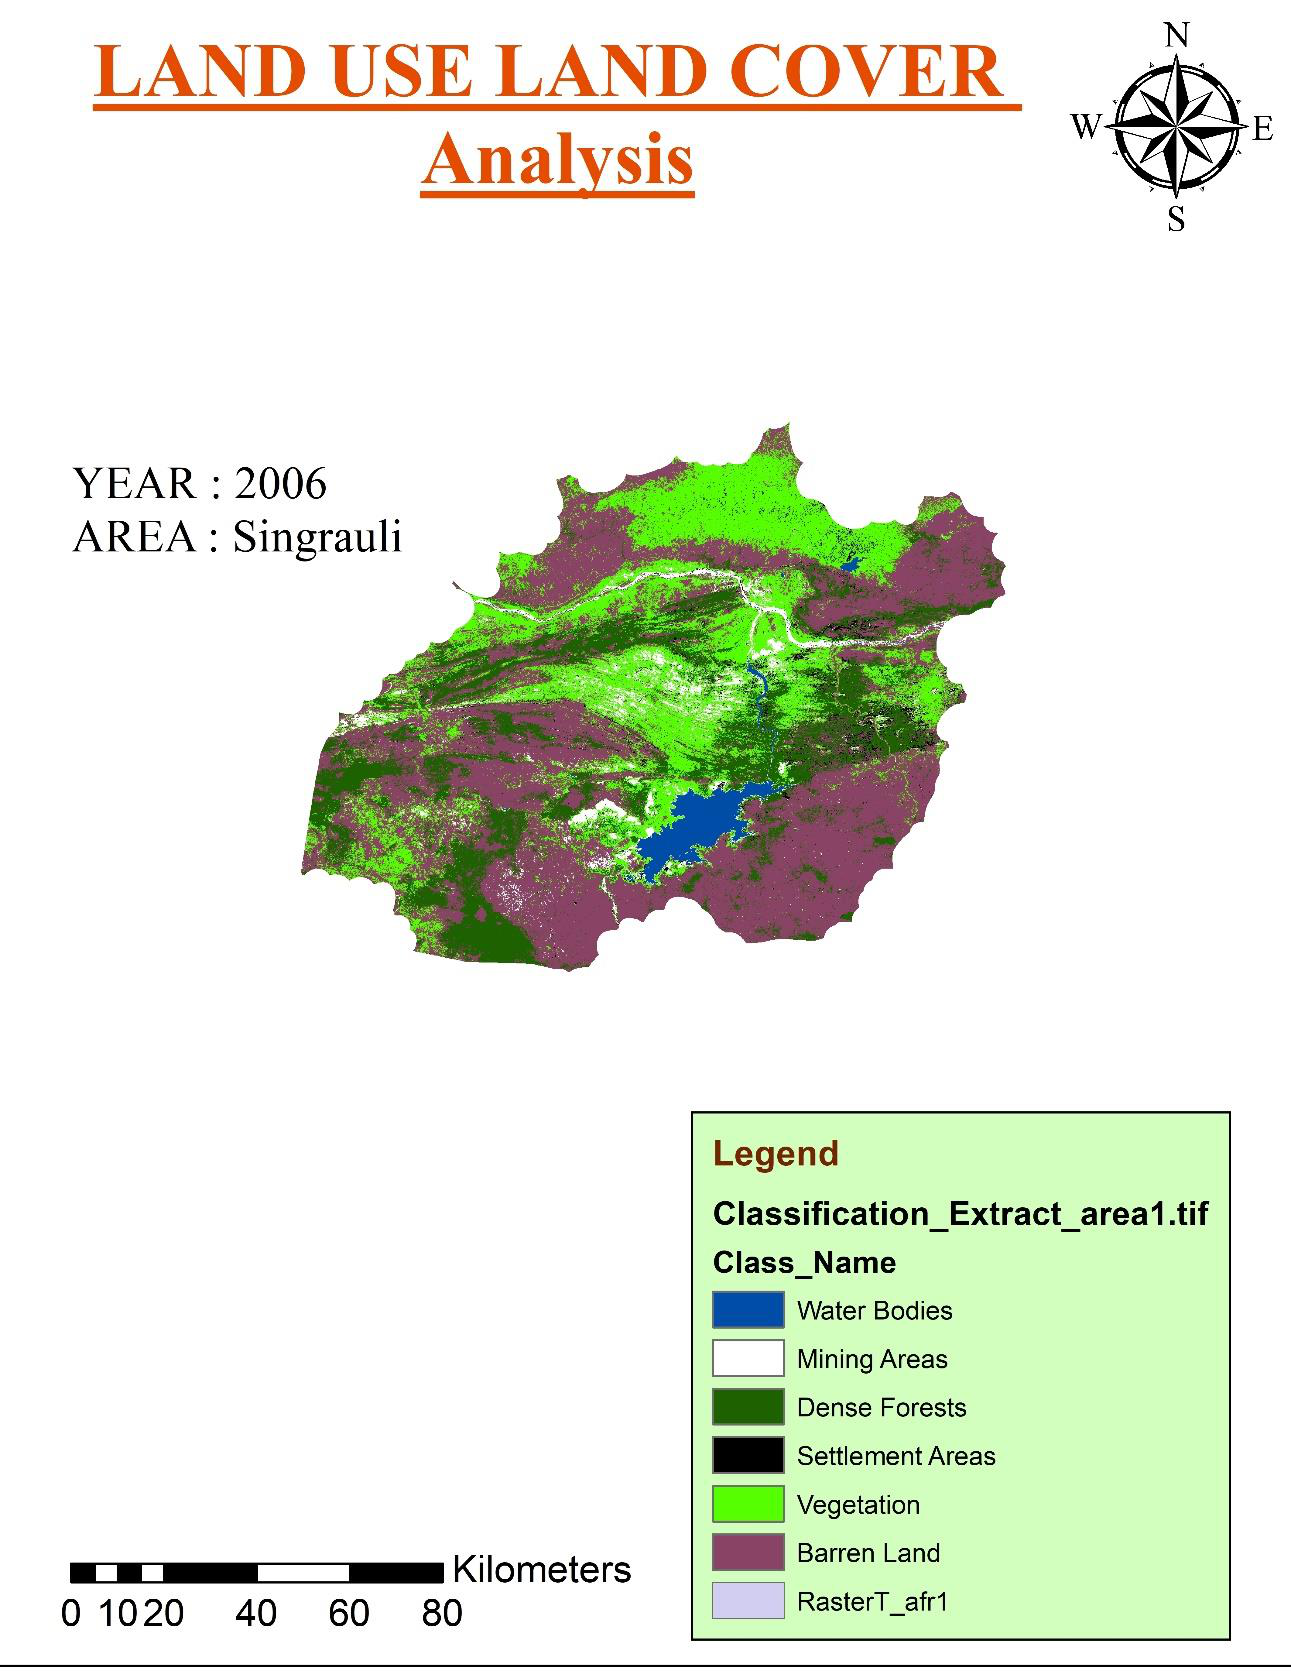
\includegraphics[width=0.85\textwidth]{fig_lulc_2006.png}
\caption{Land use / land cover map of Singrauli, 2006.}
\end{figure}

\begin{figure}[H]
\centering
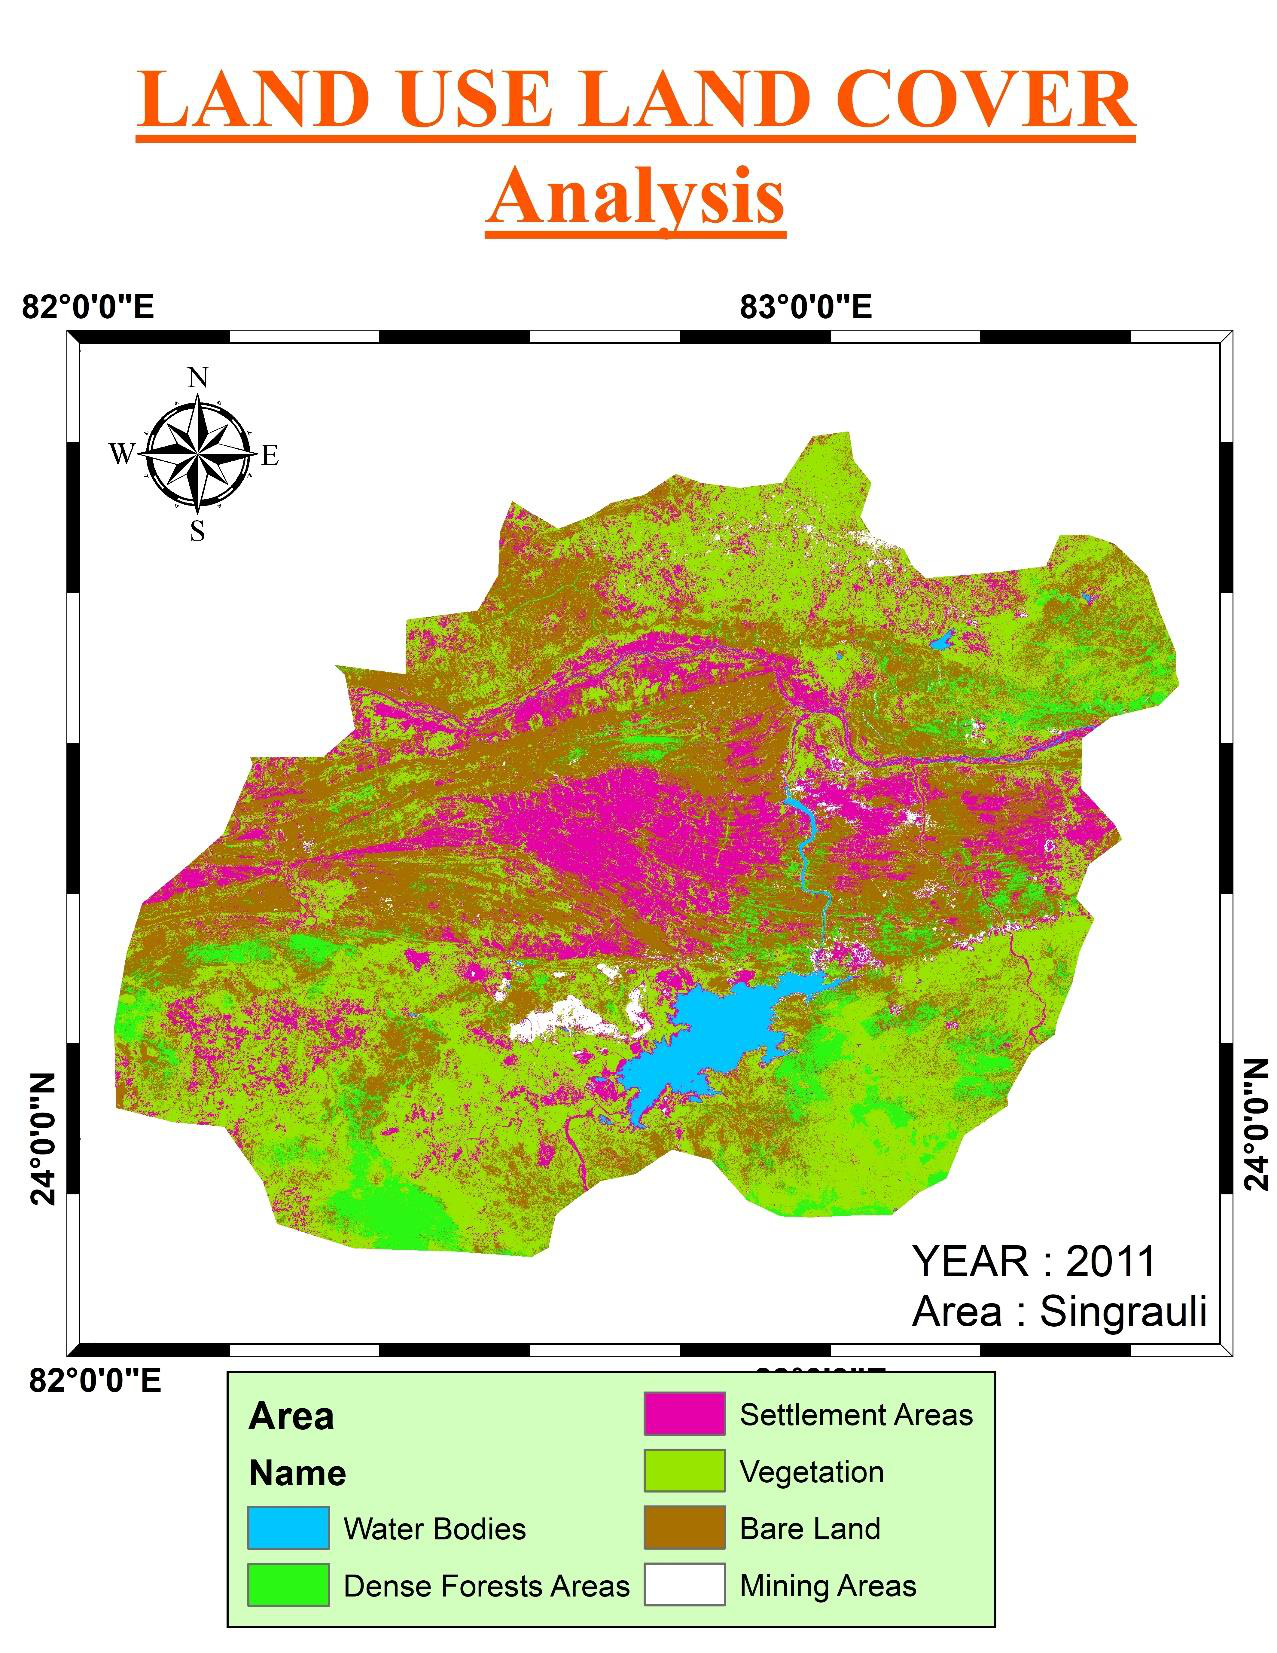
\includegraphics[width=0.85\textwidth]{fig_lulc_2011.png}
\caption{Land use / land cover map of Singrauli, 2011.}
\end{figure}

\begin{figure}[H]
\centering
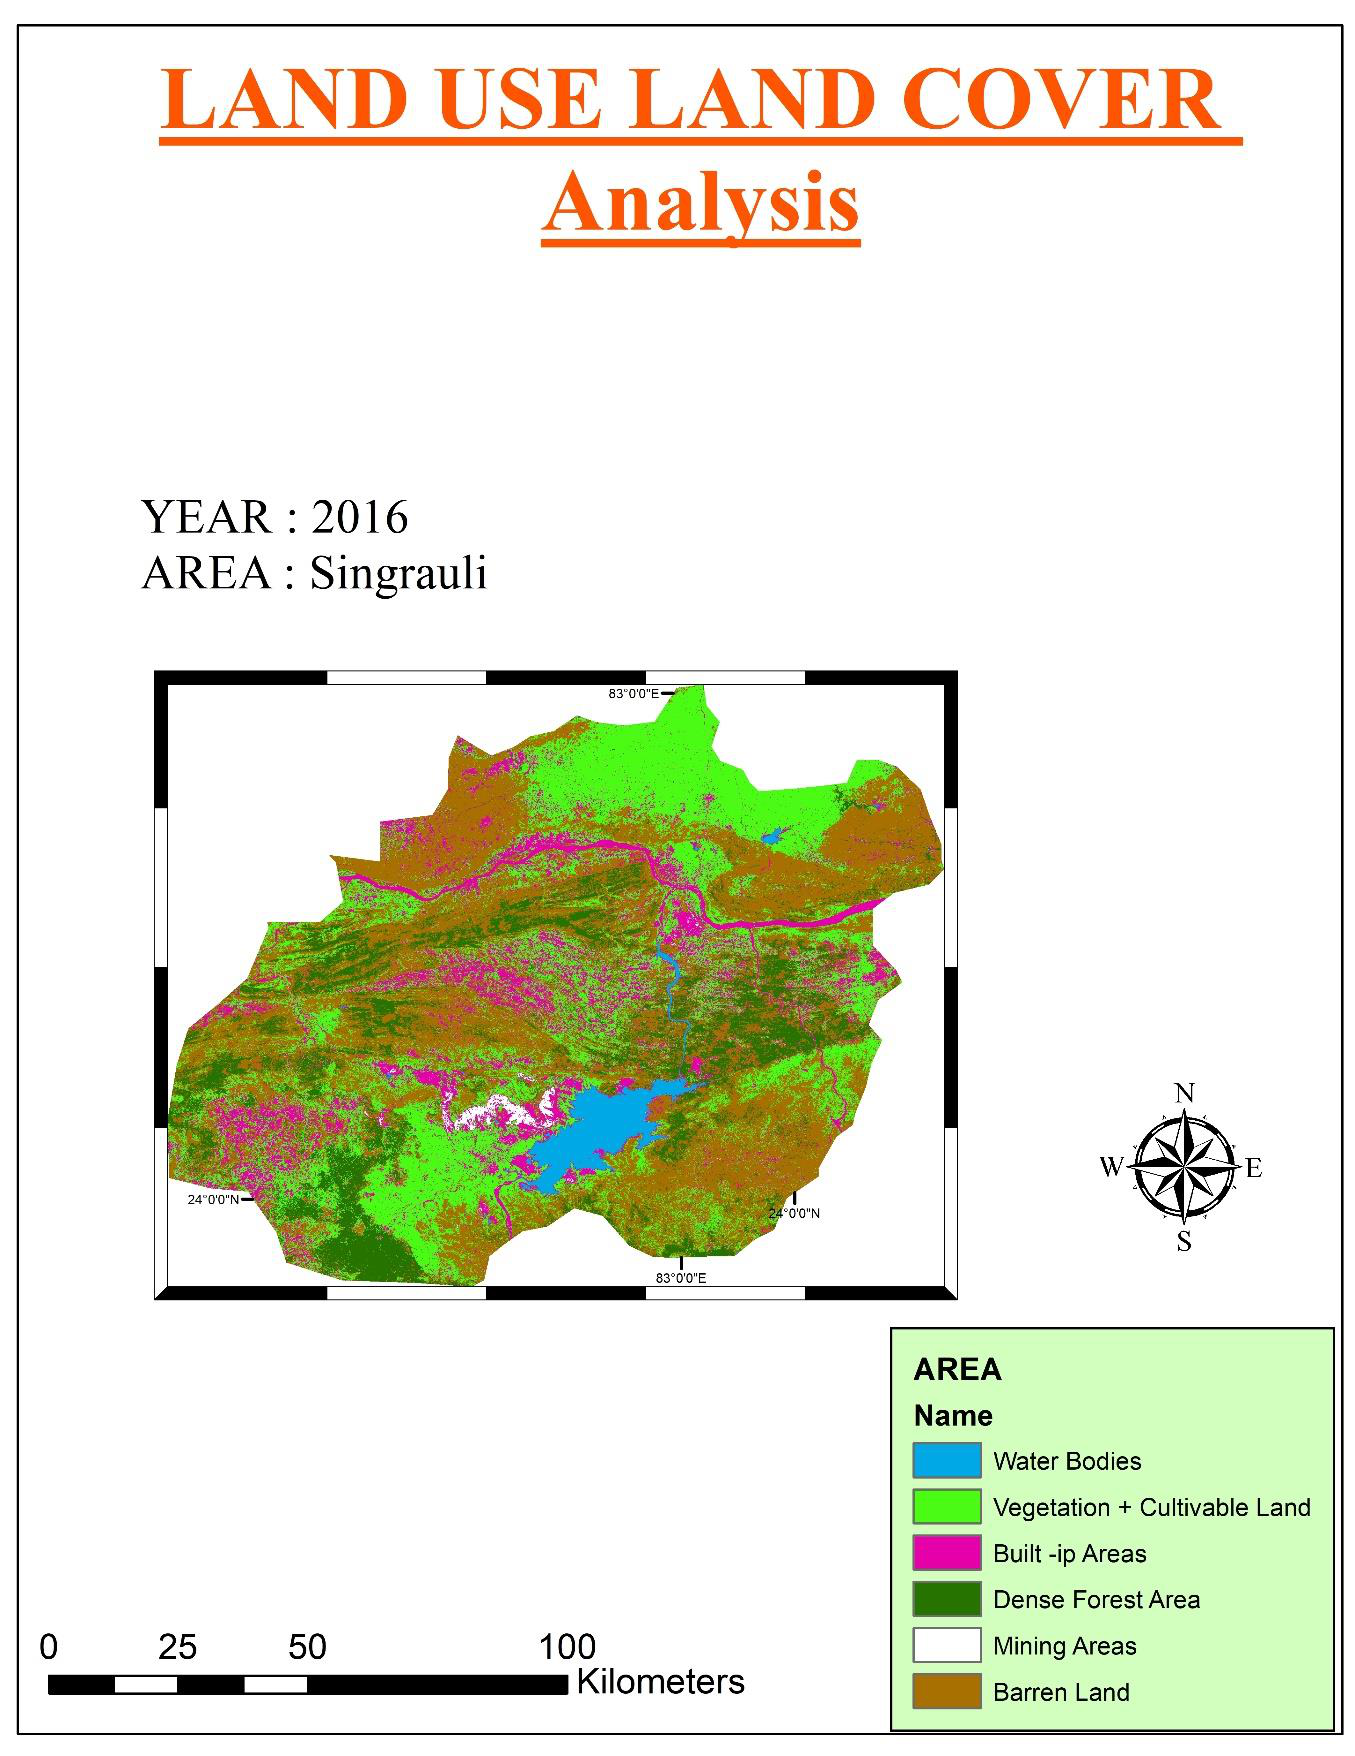
\includegraphics[width=0.85\textwidth]{fig_lulc_2016.png}
\caption{Land use / land cover map of Singrauli, 2016.}
\end{figure}

\begin{figure}[H]
\centering
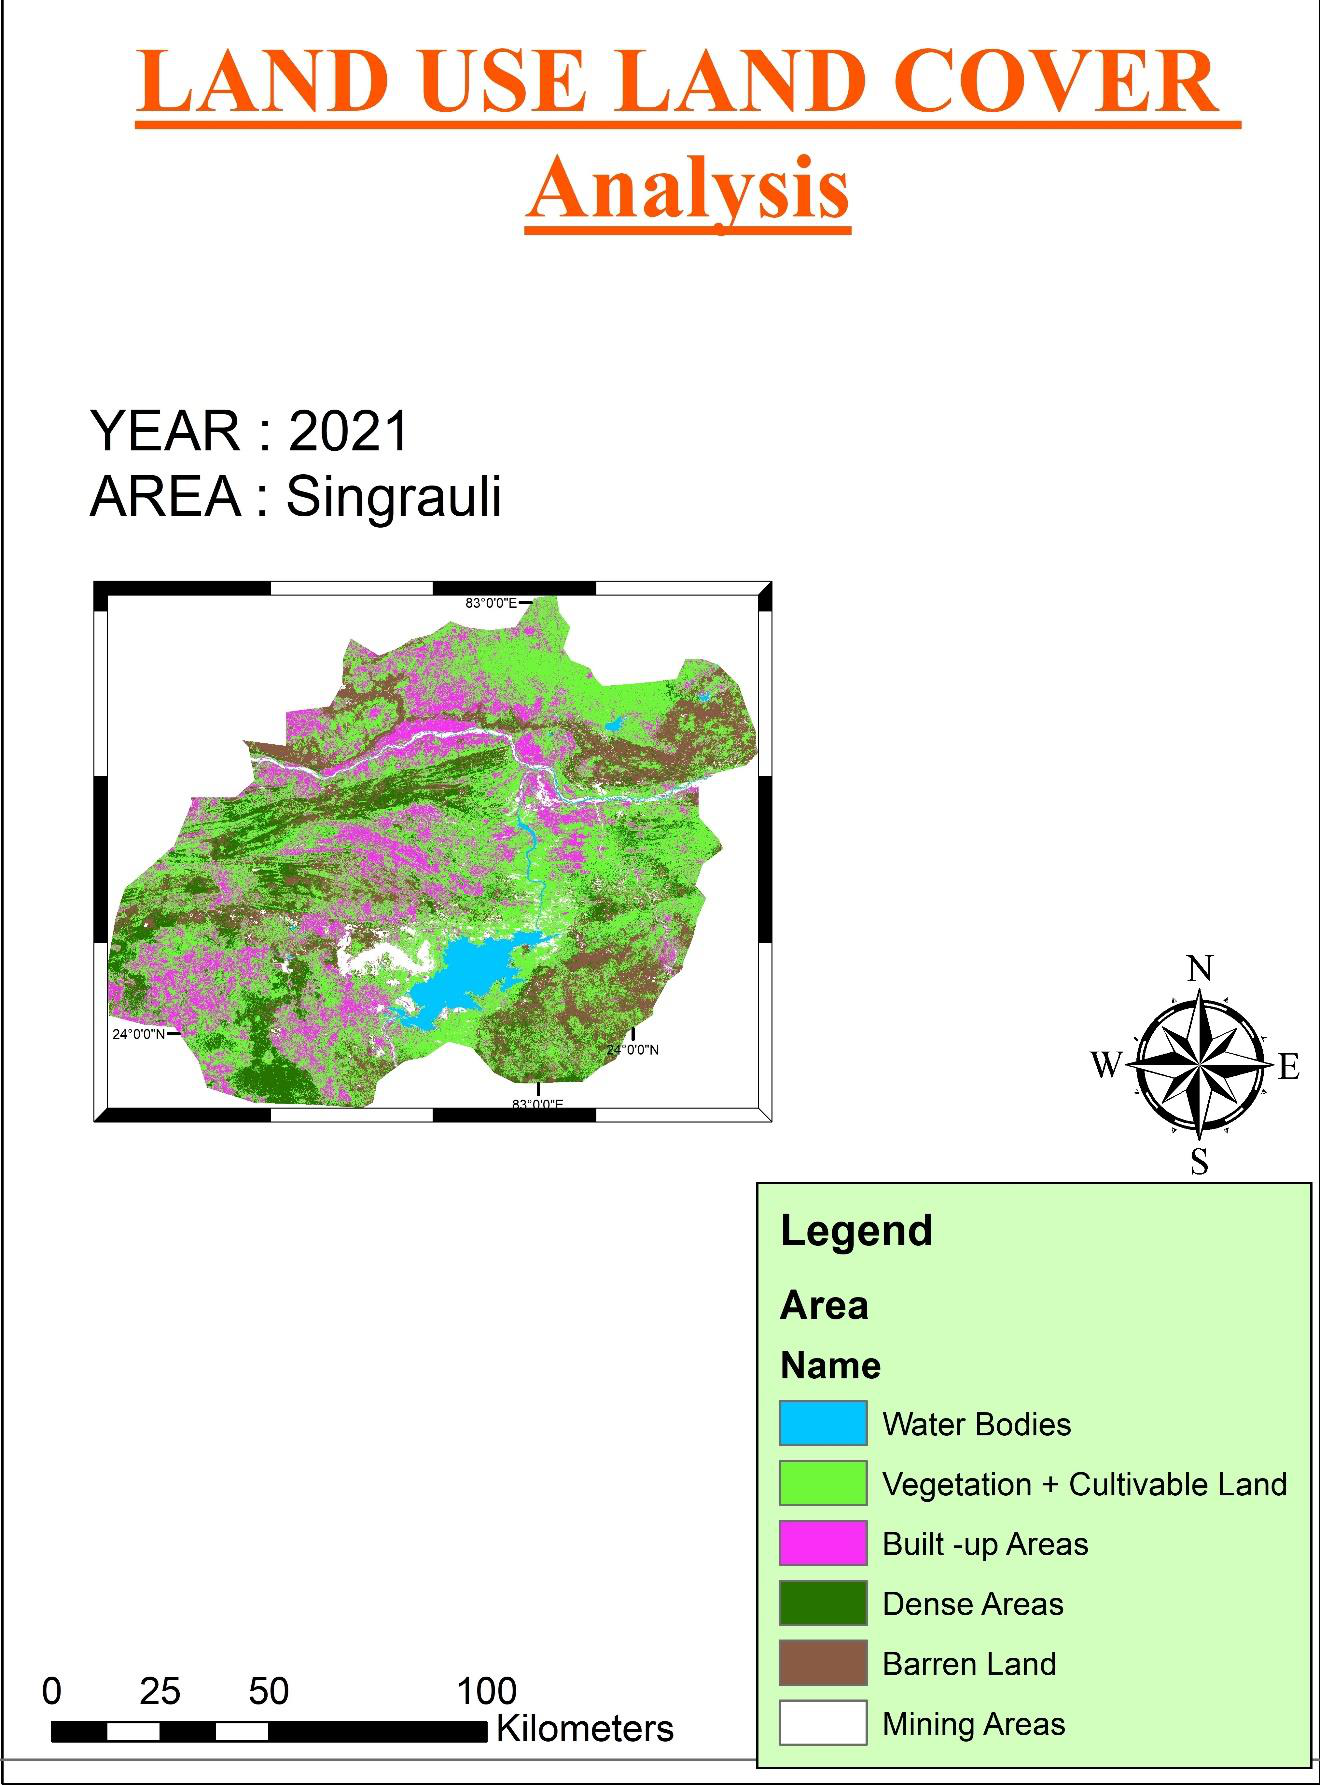
\includegraphics[width=0.85\textwidth]{fig_lulc_2021.png}
\caption{Land use / land cover map of Singrauli, 2021.}
\end{figure}

\begin{table}[H]
\centering
\caption{Percentage distribution of land use / land cover classes, Singrauli study area
(2006--2021).}
\label{tab:lulc}
\begin{tabular}{lrrrr}
\toprule
\textbf{Land Cover Class} & \textbf{2006 (\%)} & \textbf{2011 (\%)} & \textbf{2016 (\%)} & \textbf{2021 (\%)} \\
\midrule
Barren Land               & 38.71 & 32.19 & 32.16 & 15.25 \\
Vegetation + Cropland     & 23.95 & 38.48 & 38.48 & 52.62 \\
Dense Forest Areas        & 17.94 & 7.12  & 5.67  & 4.53  \\
Built-up Areas            & 16.33 & 18.43 & 23.17 & 23.84 \\
Mining Areas              & 0.58  & 1.45  & 0.21  & 3.11  \\
Water Bodies              & 2.49  & 2.33  & 0.31  & 0.65  \\
\bottomrule
\end{tabular}
\end{table}

The distribution confirms the trends discussed above: a steady decline in dense forest and
barren land, a corresponding rise in vegetation/cropland and built-up area, and a mining-area
share that, while small in absolute percentage terms, grew considerably relative to its 2006
baseline.

\section{Conclusion}

From this study, it may be concluded that a considerable amount of land cover change has taken
place in the Singrauli coalfield over the 15-year span from 2006 to 2021. Large-scale coal
mining operations have significantly altered the pre-mining environment; the area under mining
shows an increase attributable to the rapid growth in coal production, and while dense forest
area is decreasing, plantation efforts at overburden dumps under reclamation schemes have also
been ongoing. Overall, the land use/land cover change observed in the Singrauli coalfield has
resulted from the rapid expansion of mining and industrial activity during this period,
producing drastic changes in the land cover dynamics of this fragile ecosystem.

\section*{Acknowledgement}

I would like to express my deep and sincere gratitude to my research supervisor, Dr.\ Medha Jha,
for giving me the opportunity to research the topic ``Land Use Land Cover Classification of
Singrauli District'' and for providing valuable guidance throughout this exploratory project. It
was a privilege and an honour to work and study under her guidance. Special thanks are also due
to PhD student Sheela for her support during this work.

\end{document}
